% =================================快捷键及注意事项================================
%1. 注释
%"Ctrl" + "T"
%2. 去除注释
%“Ctrl” + "U"
%*************************** 用github 提交时,只提交你修改的相关文件。日志等不提交。
\documentclass{mcmthesis}
% =================================原始控制页模板设置=======================================
\mcmsetup{CTeX = true,   % 使用 CTeX 套装时,设置为 true
        tcn = 89760, problem = B,
        sheet = false, titleinsheet = true, keywordsinsheet = true,
        titlepage = false, abstract = true}
\usepackage{palatino}
\usepackage{caption} % 图片
\usepackage{subfigure} % 图片
\usepackage{lipsum} % 文本
\usepackage{booktabs} % 表格
\usepackage{makecell} % 表格线段的粗细
\usepackage{supertabular} % 多页表格
\usepackage{float} % 去除图片浮动
\usepackage[numbers,sort&compress]{natbib} % 引入多个参考文献
\setlength{\parskip}{0.2em} %设置行距
\usepackage{indentfirst}
\usepackage{slashbox}
\newcommand{\upcite}[1]{\textsuperscript{\textsuperscript{\cite{#1}}}} % 引用上标
\setlength{\parindent}{2em}
\bibliographystyle{plain}
% =================================自制控制页设置=======================================
\newcommand{\newteamnumber}{89760} 
\newcommand{\newproblemchosen}{B} 
\newcommand{\ourtitle}{Camping on the Grand River} 
% =================================自制控制页设置=======================================
\title{Camping on the Grand River} % 标题
\author{\small \href{http://www.latexstudio.net/}
  {\graphics[width=7cm]{mcmthesis-logo}}}
\date{\today}

\begin{document}
% =================================正文设置=======================================
\begin{abstract}
\noindent If an alien came after 50 years, what language should it learn to understand human civilization more fully? The research findings in this article can give an answer.
\par In this article, we predict trends in the mainstream languages of the world today and determine the address of a new international office for a multinational corporation.
\par The first stage: from the total number of language population and geographical distribution of language to predict the trend of global language development.For the former, we assume that there is no sudden factor to change the number of language speakers in a certain region drastically. Since there is a missing value in the collected data, a non-equidistant GM (1,1) prediction model is established to predict the total number of language speakers.Then analyses the trend of the total population in the first 20 languages.For the latter, consider the impact of the two factors of geographical population growth and population migration on geographical distribution of languages. 
\par The second stage: the establishment of language performance evaluation model (LII model) to determine the location of the new international offices.The LII model considers the specific 15 indicators of a language group in five major areas: Area, Economic strength, Language speakers, Knowledge and communication, International use. Firstly the indicator value is quantified to [0, 1], then weighted to obtain the language performance score and ranked.Analyze change of rankings of language performance score every 10 years in the future, and find that there is no change in the categories of the top 6 languages in terms of short-term or long-term.We assume that the offices are usually established in the capital of the country where the first language is the mother tongue, so six new offices are located: London, England / Paris, France / Madrid, Spain / Dammam, Saudi Arabia / Moscow, Russia / Berlin, Germany.Finally, considering the nature of the change in the global communications (geographically distant Internet connections and language barrier with powerful translation software), we think it is possible to set up an international office in each continent, that is, in addition to the United States and China , Confirming the establishment of four more new international offices. 	

\begin{keywords}

\end{keywords}
\end{abstract} % 模板自带的摘要
%\newgeometry{left=2.5cm,right=2.5cm}
 %==========================================以下不要动=================================================

  \pagestyle{empty}%
  \null%
  \vspace*{-6pc}%
  \begin{center}
  \begingroup
  \setlength{\parindent}{0pt}
     \begin{minipage}{0.28\linewidth}
      For office use only\\[4pt]
      \makebox[0.15\linewidth][l]{T1}\rule[-2pt]{0.85\linewidth}{0.5pt}\\[4pt]
      \makebox[0.15\linewidth][l]{T2}\rule[-2pt]{0.85\linewidth}{0.5pt}\\[4pt]
      \makebox[0.15\linewidth][l]{T3}\rule[-2pt]{0.85\linewidth}{0.5pt}\\[4pt]
      \makebox[0.15\linewidth][l]{T4}\rule[-2pt]{0.85\linewidth}{0.5pt}
     \end{minipage}%
     \begin{minipage}{0.44\linewidth}
      \centering
      Team Control Number\\[0.7pc]
      {\LARGE\textbf{\newteamnumber}}\\[1.8pc]
      Problem Chosen\\[0.7pc]
      {\Huge\textbf{\newproblemchosen}}
     \end{minipage}%
     \begin{minipage}{0.28\linewidth}
      For office use only\\[4pt]
      \makebox[0.15\linewidth][l]{F1}\rule[-2pt]{0.85\linewidth}{0.5pt}\\[4pt]
      \makebox[0.15\linewidth][l]{F2}\rule[-2pt]{0.85\linewidth}{0.5pt}\\[4pt]
      \makebox[0.15\linewidth][l]{F3}\rule[-2pt]{0.85\linewidth}{0.5pt}\\[4pt]
      \makebox[0.15\linewidth][l]{F4}\rule[-2pt]{0.85\linewidth}{0.5pt}
     \end{minipage}\par
     \vskip 8pt
  \rule{\linewidth}{0.5pt}\par
%  \vskip 8pt
  \vskip 4pt
  \textbf{{\Large\the\year}\\%
%  Mathematical Contest in Modeling (MCM/ICM) Summary Sheet}%
  MCM/ICM \\
  Summary Sheet}%
%  \par
  \endgroup
%  \vskip 8pt
 \vskip 4pt
  \normalfont \Large \ourtitle \par
%  \par
  \centering {\normalsize{\textbf{summary}}}
  \end{center}
%==========================================以上不要动=================================================

% ============================================摘要======================================================
\noindent If an alien came after 50 years, what language should it learn to understand human civilization more fully? The research findings in this article can give an answer.
In this article, we predict trends in the mainstream languages of the world today and determine the address of a new international office for a multinational corporation.
In the first stage: In the first stage, forecasting trends of global languages takes two aspects into account: the change in the total number of people in a particular language and the geographical distribution of the language. For the former, a non-equidistant gray prediction model based on historical data is established under the assumption that there is no sudden change in the number of language speakers in a region.The model gives the number of speakers of the language (ranked in the top twenty).For the latter, we consider the language speakers' geographic distribution.At this time, the influence of the regional population growth and population migration on the shift is taken into account. By applying these two models, we can obtain the change of the total number of speakers of the mainstream languages in the world(Shown in Fig.), the variations of the number of native speakers in the mainstream languages(Shown in Fig.),languages of top ten(both native speakers and total speakers) and their ranks in fifty years(see table).Additionally, we find none of the top ten languages of both native speakers and total speakers is replaced in fifty years and English becomes the most spoken language by the year 2045 with a total population of 1,432.163 million.As for the part of geographical distribution of language speakers,we obtain that the Arabic speakers accounts for 50.13% of the total Arabic speaker in 2048.,which indicates geographical distribution of Arabic speakers skews toword AfricaFrench also shows the same trend.
In the second stage: the establishment of language performance evaluation model (LII model) to determine the location of the new international offices. The LII model considers the specific 15 indicators of a language group in five major areas: Area, Economic strength, Language speakers, Knowledge and communication, International use. Firstly the indicator value is quantified to [0, 1], then weighted to obtain the language performance score and ranked. Analyze change of rankings of language performance score every 10 years in the future, and find that there is no change in the categories of the top 6 languages in terms of short-term or long-term. We assume that the offices are usually established in the capital of the country where the first language is the mother tongue, so six new offices are located: London, England / Paris, France / Madrid, Spain / Dammam, Saudi Arabia / Moscow, Russia / Berlin, Germany. Finally, considering the nature of the change in the global communications (geographically distant Internet connections and language barrier with powerful translation software), we think it is possible to set up an international office in each continent, that is, in addition to the United States and China , Confirming the establishment of four more new international offices.




% ============================================摘要======================================================

% ============================================下面关键字======================================================
\par
\noindent
\textbf{Key words:}Non-equal spacing GM (1,1) ,Evaluation model of language effectiveness 
 % 控制页及摘要 
\restoregeometry % 恢复原来的设置
\maketitle  % 模板自带:添加
\tableofcontents % 添加目录
\newpage % 段页
% =================================子文件夹设置====================================
% 在子文件夹下编写文件
\section{Introduction}

\subsection{Background}
\noindent
There are currently about 6909 languages in the world, and the total number and geographical distribution of each language is a necessary consideration for international organizations and economic development. The so-called language population refers to the native language of the population \upcite{cinemaData}. In the analysis of the number of native speakers of the world language, nearly half of the population is native speakers in the following 10 languages: Mandarin (incl. Standard Chinese), Spanish, English, Hindi, Arabic, Bengali, Portuguese, Russian, Punjabi, and Japanese.

However, many people use this as their second language. The total number is not determined solely by the number of native speakers,that can determine the total number of 0.4~0.8. For a language as a second language or a third language or even more, the number of people in order and the order of the mother tongue is not the same arrangement. Therefore, when analyzing the trend of global language use, we should not only consider the number of native speakers, but also the change of the number of  second and third languages as non-native speakers. 

Over time, the increase or decrease in the total number of uses of a language is influenced by a number of factors. These factors are broadly divided into policy factors: the official language of a government or the promotion of a language, educational factors: the language of school teaching, social factors: employment pressure, cultural factors: cultural diffusion and assimilation phenomenon, demographic factors: the country's demographic changes and migration led to population migration. At the same time, due to the rapid development of the global economy, the increase of international business and transnational corporations, economic factors can drive the influence of a country's language and thus the total number of people who use language.Now the internet is popular, the world is closely related, the use of communication media and the help of mobile software, such as accurate and rapid language translation and other network factors can also affect the development of language. These factors may have an impact on the trend of language development, but not just that. 
\subsection{Restatement of the problem}
\noindent
We are required to investigate trends of global languages,and provide a multinational service company with a new international office location plan.
\par We understand the problem as follows:

	\begin{itemize}
		\item
We are asked to set up a model to describe the distribution of language over time based on possible influencing factors.
		\item
We should predict how the number of native speakers and total speakers will change in the next 50 years and whether the top 10 native speakers and total speakers will be replaced by another language.
		 \item
Based on the world population growth and immigration patterns for the next 50 years, we need to determine whether the geographical distribution of the language will change during this period. If so, describe the change.
		 \item 
Provide international service companies with site selection plans for new offices and consider whether the programs will be different from the perspective of long-term and short-term.
		\item 
Given the changing nature of global communications, in order to reduce the number of new international offices, we are supposed to consider additional information and give further advice based on additional information.Finally, we were also asked to write a memorandum to the relevant department. 		 	 
	\end{itemize}



\subsection{Our works}
When predicting the of language, two key factors should be taken into account: the change of the total population in a given language and the geographical distribution of the language. These two factors determine the number and spatial distribution of language speakers, so we need to look at how these two factors change over time. The dominant language of the geographical area to be selected to construct a new International Office should have great international influence, more appropriately, its effectiveness. Therefore, we must make a quantitative assessment of the effectiveness of the language. Our work is completed in the following steps:

\begin{itemize}
	\item 
	Determine how the number of language speakers changes over time. Due to the large roughness and incompleteness of the existing statistical data, we established a non-equidistant gray prediction model. Applying this model,we eliminate the randomness of collected data and predict how the number of language speakers changes.
	\item Ascertain the transformation in the geographic distribution of the language speakers. We consider the change of geographical distribution of native and second languages. Define population concentration to determine the geographical transfer of the native speaker distribution center.We consider the mode of immigration to determine the spatial shift in the second language. Combining the above two parts we can get the trend of the mainstream languages and the geographical distribution of each language,and we can determine the language rankings and their changes in the next 50 years. 
	\item Evaluate the effectiveness of the language. We establish the evaluation model of the international influence of language in order to determine the effectiveness of the language. Based on the language's score given by the above model, the language area for the new international office is determined. Finally, we follow consideration of the rapid development of the Internet and global social media. We suppose that we can capture the penetration of regional Internet and that the multinational companies have web services.If so, We can regard the level of Internet penetration in a region as a guideline for the need to establish an office there. That is the higher the Internet penetration rate in a given area, the lower the need to have an office there, since the company can handle the business through its network channels
	
\end{itemize}


\subsection{Conceptual Analysis}

\begin{itemize}
	\item \textbf{Native language and second language}
	\par In 1951, UNESCO convened a meeting on the mother tongue in Paris and defined the mother tongue as follows: "Mother tongue refers to the language a person learns from an early age and is usually a natural tool for his thinking and communication.The second language refers to a person who, besides the first language, learns and understands the second language, often as an auxiliary language and a common language.
	\item \textbf{Second language and foreign language}
	\par The difference between a second language and a foreign language often depends on education. Although neither is born speaker, the former refers to the language that possesses context during the learning phase, the latter usually refers to a language that lacks context during the learning phase.
	For example, in China, English has been ever more common, and attractions, media and airports have English. However, China does not entirely popularize English context. Therefore, English continues to be a foreign language, not a second language. As in Egypt, English is also a foreign language.
\end{itemize} % 介绍
\section{Analysis of Overall and Key Points}
\noindent In the first part of the question, two key points should be considered in predicting trends of global languages: the total population change in a given language and the geographical distribution of the language. In the section on simulating changes in total population speaking a center language, we need to collect historical data on changes in the number of language speakers. Next, we determine the geographical distribution of languages. To simulate the geographical distribution of the population using different languages, we consider two key factors: the change in the number of people using a language in the world and the immigration situation. For the former, we can analyze the deviation of the population center in speaking the language by comparing the changes in the number of people in the same language but in different regions. For the latter, we establish a migration model to simulate immigration, which gives the geographical distribution changes of the language caused by the immigrants.
\par In the second part of the question, when locating an international office, the effectiveness of the local language should be taken into account, namely the usefulness of the language. To take an extreme example, if a Martian descends upon Earth, what language should a Martian learn to understand the Earth as much as possible, and English is the most suitable language for now. So we propose an evaluation model of the effectiveness of languages in the future, according to which we can rank the language based on its effectiveness and determine where international offices should be constructed on the ranking results. % 模型的分析
\section{Assumptions and Justification}

\begin{itemize} 
	
    \item \textbf{Do not consider unexpected factors such as war factors. }We assume that some local language will not disappear due to other unexpected factors such as war. Since the probability of such an incident is minimal, we do not consider it.
    
    \item \textbf{Suppose the data collected is reliable .}Since most of the data we collect comes from the United Nations statistics, we consider these data to be reliabl.
    
    \item \textbf{Suppose the population using lower-ranked languages will not surge.}With the total population as the ranking criterion, the top 20 languages have the potential to enter the top 10, and considering the lower-ranked languages thave small population base,we ignore them.
    
    \item \textbf{Ignores the impact of policy on language distribution.} Due to the great uncontrollability and unpredictability of government policy making, this model does not consider the influence of government policy on language distribution.
    
    \item \textbf{When considering the mode of population migration, government intervention in population movements is ignored.}The immigration policy implemented by a government is related to numerous factors such as the demographic structure of each stage of our country and international partnerships. As a result, there is a great deal of uncertainty in the policy. Therefore, simplifying the analysis does not consider the policy factors.
    
	
\end{itemize}  % 假设
\section{Symbols and Definitions }
\noindent
In the section, we use some symbols for constructing the model as follows: 
%==============================================================================
% 在最后的排版中如果一页放不下,可以分开放。
\begin{table}[H]
	\begin{center}
		\caption{\label{tab:Symbols_total}Symbols and Definitions}
			\renewcommand\arraystretch{1.5}
				 \scalebox{0.87}[0.87]{%
		\begin{tabular*}{35em}{ c p{12cm}}
			\toprule
		 Symbol  & Definition \\
		 \midrule
    	${x_m}^{(0)}({k_n})$&  The total population of the m-th language using that language in year \\
			$L{1_i}^j$	 & The number of native speakers in the language region Community  using the j-th language\\
			${\gamma _i}$	 & The extent to which a language is localized in a language region\\
			$P_i^j$	 & Number of net movers in a country's second language \\
			$L2_i^j$	 & Number of assimilated people in a language zone\\
			$m$	 &The m-th indicator \\
			${\omega _m}$	 & The weight of each indicator\\
			$S_m^j$	 & The m-th indicator normalized the result\\
			${s^j}$	 & Total score of international influence in the j-th language\\
			\bottomrule
		\end{tabular*}
	}
		\renewcommand\arraystretch{1}
	\end{center}
\end{table}

 %符号设置
\section{Models}

\subsection{the tendency of language speakers}
\noindent There are two keys to be considered about the language trends: the change in the number of language speakers and their geographical distribution. The key to studying the change in the number of speakers is to build a sound predictive model. Considering the incompleteness and roughness of the statistical data about speakers, we consider the establishment of a non-equidistant gray prediction model. In considering the geographical distribution of language speakers, we study the following two aspects: the regional disparities in the distribution of the language speakers in different regions and the changes in the geographical distribution of second languages due to immigration.

\subsubsection{Changes in the number of language speakers}
\noindent For the study of the trend of global language change, we should consider two aspects, that is, the change in the total population of a certain language and the change in geographical distribution of language speakers, As explained in the Problem Analysis, when predicting trends in the population of languages, we first need to collect historical data about the particular language being used.The data are listed below:


\begin{table}[H]
	\centering
	\caption{Global rankings in 2014, 2015, 2016, 2017 Change in total headcount usage in the top 23 languages}
		 \scalebox{0.87}[0.87]{%
	\begin{tabular*}{35em}{@{\extracolsep{\fill}}clrrrr}
		\toprule
		\multicolumn{1}{l}{Number} & Language & 2014  & 2015  & 2016  & 2017 \\
		\midrule
		1     & Chinese,Mandarin & 1052.535 & 1070.966 & 1073.525 & 1076.734 \\
		2     & Spanish & 441.7462 & 453.7809 & 466.8536 & 480.4602 \\
		3     & English & 816.9127 & 903.37 & 911.6737 & 917.9667 \\
		4     & Hindi & 365.4672 & 365.735 & 366.4932 & 367.5688 \\
		5     & Portuguese & 196.7223 & 198.126 & 200.7203 & 202.5036 \\
		6     & Bengali & 184.1833 & 186.2771 & 183.2275 & 179.4995 \\
		7     & Russian & 189.6124 & 192.1039 & 194.2471 & 197.3681 \\
		8     & Japanese & 124.9867 & 125.1537 & 125.3209 & 125.5303 \\
		9     & Javanese & 77.36284 & 76.93927 & 76.51803 & 75.99483 \\
		10    & German,Standard & 146.0954 & 146.6092 & 147.6057 & 148.2428 \\
		11    & Chinese,Wu & 73.22911 & 72.48929 & 71.75694 & 70.85228 \\
		12    & Korean & 117.8224 & 117.8665 & 117.9106 & 117.9658 \\
		13    & French & 126.9646 & 153.8068 & 154.9492 & 155.939 \\
		14    & Telugu & 81.37525 & 81.70919 & 82.14315 & 82.18562 \\
		15    & Marathi & 71.41339 & 71.47918 & 71.54502 & 71.62742 \\
		16    & Turkish & 58.45415 & 58.32959 & 58.2053 & 58.05032 \\
		17    & Tamil & 73.58453 & 73.5565 & 73.52849 & 73.4935 \\
		18    & Vietnamese & 67.34071 & 67.26303 & 67.18545 & 67.0886 \\
		19    & Urdu  & 153.8177 & 153.5716 & 153.3494 & 153.0674 \\
		20    & Italian & 64.94941 & 64.9459 & 64.94238 & 64.93799 \\
		\bottomrule
	\end{tabular*}%
}
	\label{tab:addlabel}%
\end{table}%

 The table above shows the changes in the total number of people speaking the top 23 languages in the world in 1999, 2009, 2014, 2015 and 2017.
 
 We analyze the data in the above table and consider the small amount of data (only four years of data), while the Gray Prediction Model has the characteristics of less input data but high prediction accuracy. And driven by reference\upcite{gm11}, we establish a non-equidistant Gray Prediction Model GM (1,1) to predict the number of language speakers.Due to the non-equidistant distribution of data over time, we define non-equally spaced sequences of language speakers:



\begin{equation}
\begin{aligned}
& {x_j}^{(0)}({k_i}) = \left\{ {{x_j}^{(0)}({k_1}),{x_j}^{(0)}({k_2}),...,{x_j}^{(0)}({k_n})} \right\} \\
& \qquad \qquad \qquad \Delta {k_i} = {k_i} - {k_{i - 1}} \\
\end{aligned}
\end{equation}

\par where, ${x_j}^{(0)}({k_i})$ represents the sequence of changes in the number of speakers in the m-th language over time, ${x_j}^{(0)}({k_n})$  is the total number of people who speak the $j$-th language in ${k_i}$ year ,(where n = 4), which corresponds to four years in the historical data. Obviously $\Delta {k_i}$  is not a fixed value here. Because we have only four sets of data, which contains very little system information,. In order to strengthen its regularity, we will do Accumulated Generating Operation on it, the result of a cumulative sum is defined as AGO of the non-equally spaced sequence ${x_j}^{(0)}({k_i})$ , marked as

\begin{equation}
{x_j}^{(1)}{\rm{(}}{k_i}{\rm{) = }}\left\{ {{x_j}^{(1)}({k_1}),{x_j}^{(1)}({k_2}),...,{x_j}^{(1)}({k_n})} \right\}\label{aa1}
\end{equation}

Where ,  makes the following formula true 

\begin{equation}
{x_j}^{(1)}{\rm{(}}{k_i}{\rm{) = }}\sum\limits_{m = 1}^i {{x_j}^{(0)}({k_j})\Delta {k_j}{\rm{ ,  }}} i = 1,2,...,n
\end{equation}

Based on the above, the steps of using non-equidistant Gray Prediction Model\upcite{gm11} to predict the number of speaking speakers over the next 50 years are as follows:

 \begin{enumerate}
 \item[\textbf{Step1}]  Determine the interval of non-equally spaced sequences.
 \item[\textbf{Step2}] From the formula (1) to generate a cumulative sequence.
 \item[\textbf{Step3}] Least square method is used to determine the parameters a\&b to be identified in the albinism differential equation ,that is
		 \begin{equation}
		 \phi {\rm{ = }}\left[ {\widehat a\widehat b} \right] = {({B^T}B)^{ - 1}}{B^T}Y 
		 \end{equation}
	where, $B{\rm{ = }}\left[ {\begin{array}{*{20}{c}}
		{{z_m}^{(1)}({k_1})}1\\
		\vdots  \vdots \\
		{{z_m}^{(1)}({k_n})}1
		\end{array}} \right]$, $Y{\rm{ = }}({x_j}^{(0)}({k_2})\Delta {k_2},{x_j}^{(0)}({k_3})\Delta {k_3}, \cdots ,{x_j}^{(0)}({k_n})\Delta {k_n})$ and ${z_j}^{(1)}({k_i})$  is the background value \upcite{influential} of ${x_j}^{(1)}(t)$  on the discrete interval  $\left[ {{k_i},{k_{i + 1}}} \right]$.
  \item[\textbf{Step4}] The estimate ${\widehat x_m}^{(0)}({k_{i + 1}})$ of ${x_m}^{(0)}({k_{i + 1}})$  is calculated\upcite{influential} from the parameters a, b.
\end{enumerate}

From the above derivation process, we use MATLAB (Programming code is shown in appendix) as a programming tool to determine the total number of the mainstream languages speakers in the next 10 years the results( Figure \ref{fig:next50}) are as shown below:
     

\begin{figure}[H]
	\centering
	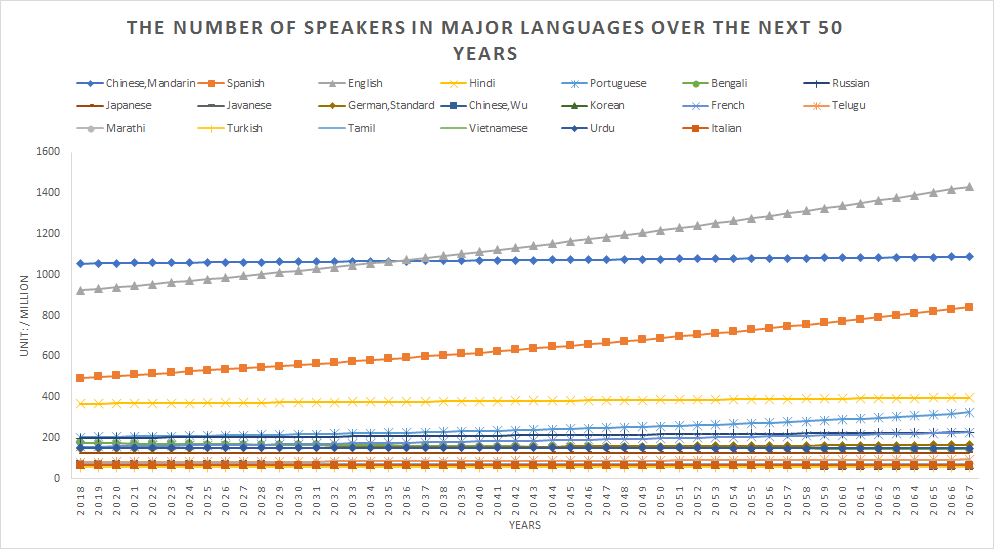
\includegraphics[width=1\linewidth,height=8cm]{figures/next50number}
	\caption{The number of speakers in major languages over the next 50 years}
	\label{fig:next50}
\end{figure}

After analyzing the figure above, we find that the total number of English-speaking population exceeded that of Chinese by 2045 and become the most heavily spoken language in the world.Additionally, the most powerful growth is in Spanish. In 2067, the rankings of the top ten mainstream languages in the world are:

\textbf{English,Chinese Mandarin, Spanish ,Hindustani, Arabic ,Portuguese, Russian, French, German Standard, Malay.}

The changes in the number of native speakers in the future areshown in the following Figure \ref{fig:percent1} :
\begin{figure}[H]
	\centering
	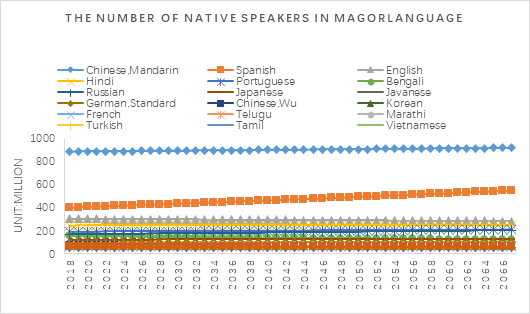
\includegraphics[width=1\linewidth,,height=8.1cm]{figures/percent}
	\caption{The number of native speakers in major language}
	\label{fig:percent1}
\end{figure}
Analyzing the figure above, we find that the number of people who speak Mandarin as their mother tongue is the largest, followed by Spanish, with the most pronounced growth trend in the language. In 2067, the top 10 languages that are speaked as the first languages are Chinese Mandarin, Spanish, English, Hindi, Portuguese, Arabic, Bengali, Russian, Japanese, German Standard.

Considering the results of the analysis of the above two graphs and comparing the current two rankings provided in the topic, we can get the following table (Table \ref{tab:Language}):


% Table generated by Excel2LaTeX from sheet 'Sheet1'
\begin{table}[H]
	\centering
	\caption{Language ranking comparison}
	\begin{tabular}{l p{2.8cm}p{2.8cm}p{2.8cm}p{3.2cm}}
		\toprule
		\multicolumn{1}{l}{Rank} & native speakers(2017 year) & native speakers(2067 year) & total speakers(2017 year) & total speakers(2067 year) \\
		\midrule
		1     & Mandarin & Mandarin & Mandarin & English \\
		2     & Spanish & Spanish & English & Mandarin \\
		3     & English & English & Hindustani & Spanish \\
		4     & Hindustani & Hindustani & Spanish & Hindustani \\
		5     & Arabic & Portuguese & Arabic & Arabic \\
		6     & Bengali & Arabic & Malay & Portuguese \\
		7     & Portuguese & Bengali & Russian & Russian \\
		8     & Russian & Russian, & Bengali & French, \\
		9     & Punjabi & Japanese & Portuguese & German,Standard \\
		10    & Japanese & German Standard. & French & Malay \\
		\bottomrule
	\end{tabular}%
	\label{tab:Language}%
\end{table}%

Our analysis of top 10 languages in 2017 and 2067 shows the following results: it is true that none of the top ten languages are replaced for both native speakers and total speakers , but the exact rankings of the ten languages change. The total number of English speakers surpassed that of Chinese. In the mother tongue, Chinese still occupy the dominant position, followed by Spain to maintain the status of second place unchanged.

\subsubsection{The impact of Population Migration on the Geographical}
\noindent
Simulating the geographical distribution of changes in the population of different languages, we consider two key factors: the change in the number of languages in the world and the immigration situation. For the former, we compare the difference in the number of the same language speakers in different regions. In that way, we obtain the transformation law of geographical distribution of the population speaking the language.And for the latter,a population-flow model is proposed to simulate immigration, which can show the change of the geographical distribution of the language caused by immigrants over time. To facilitate modeling, as described in the problem analysis, we define Asia, Europe, Africa, North America, South America, and Oceania as the six-language collective, Respectively marked as ${R_1},{R_2}, \cdots ,{R_m}$ ,where m is 6 . According to reference \upcite{gm11}, we find that more than half of the world's growing population over the next 50 years is derived from Africa. And given our time constraints, we study only in the top 20 languages in Africa (the region most likely to be the center of distribution for language speakers. Based on the results calculated from the model built in the first part of the question we chose French, Italian, Arabic, English, Portuguese as the research object.

In order to facilitate the analysis of the geographical distribution of a linguistic population over time,we define language regional collective as follows:

\begin{equation}
{\gamma _i} = \frac{{L{1_i}^j}}{{\sum\limits_{i = 1}^6 {L{1_i}^j} }}
\end{equation}

${\gamma _i}$ characterizes the degree of distribution of a language in a Language Regional Collective,.The greater the value, the greater the number of speakers of that language in this region.

After that, we compare the values of ${\gamma _i}$ in different regions and then we can get the geographical distribution differences of the studied languages.

Apply ing the data from the first part of the modeling (see Annex 1), we can get the change of the ratio of the total speakers of French, Arabic, Italian, English and Portuguese to the total speakers in these four languages in Africa. The results are shown in the following figure.

\subsubsection{Impact of Population Migration on the Geographical Distribution of Second Language}
\noindent Based on the above questions, we can draw a conclusion that the number of second language speakers in the number of changes in the trend because the world outside the mother tongue of a second language is known geographical map, combined with Google Maps Analysis of the second language used mainly as follows:

% Table generated by Excel2LaTeX from sheet 'Sheet2'
\begin{table}[H]
	\centering
	\caption{ The second language is mainly used in countries / regions}
	\begin{tabular}{llp{5cm}p{5cm}}
		\toprule
		language & Asian & Europe & Oceania \\
		\midrule
		Chinese &       &       & Australian \\
		\midrule
		English &       & Sweden, France, Iceland, Poland &  \\	\midrule
		spanish &       &       &  \\	\midrule
		Arabic &       &       &  \\	\midrule
		Russian &       &Ukraine, Kazakhstan, Uzbekistan,Turkmen&  \\	\midrule
		Bengalese & India&       &  \\	\midrule
		Portuguese &       &       &  \\	\midrule
		French &       &       &  \\	\midrule
		Hausa &       &       &  \\	\midrule
		Turkish &       & Austria,Germany, Bulgaria &  \\	\midrule
		Italian &       &       &  \\
		\bottomrule
	\end{tabular}%
	\label{tab:addlabel}%
\end{table}%

\par According to the above table and the relevant data \upcite{undata}, we can see that as the top10 of the second language of the country, the following are arranged in order (in parentheses, the number of countries): English (55), French (14), Russian (13), Spanish , Creole (8), Arabic (8), Kurdish (4), Portuguese (4), Italian (3), Quechua (3).
\par The changes in the geographical distribution of the second language mainly consider the impact of the population migration pattern, in which the migration pattern of the population is mainly influenced by government policy and emigration of a country. We simply think that no government intervention or intervention policy in a certain period of time remained basically unchanged, so we only consider the impact of immigration factors on the second language in the geographical distribution of change.According to the data, we choose to use the net migration to reflect the immigration factor. It is known that the United Nations predicts the net migration before 2100 \upcite{undata}, and at the same time it can avoid errors in the data obtained by our own prediction model.To simplify the model, we assume that the net number of new moves in a given linguistic region is proportional to the number of new speakers using the dominant language in the region as a second language,and the definition of the newly added population that dominates the region's second language as an assimilated population.
\par We can calculate the number of people who are assimilated in the language region by the number of net immigrants in a language region. As follows:

\begin{equation}
\L2_i^j{\rm{ = }}\frac{{P_i^j}}{{\sum\limits_{i = 1}^n {P_i^j} }}L{2^j}\label{aa1}
\end{equation}

\noindent Among them: $P_i^j$ represents the number of net immigrants in a country's second language, $L2_i^j$ represents the number of assimilated people in a certain language region, that is, the number of second-language growers, $L{2^j}$ represents the $j$th-language growth,this value is determined by the model of the first part of the question.
\par According to the above analysis and formula, Echarts Gallray can be used to make a dynamic map of the geographical distribution of a second language under the influence of population migration \upcite{mapdata}. The geographical distribution of second language speakers in each language in the above table can be displayed.Random screenshots here to get the number of speakers in English, Spanish as a second language in the geographical distribution of changes:

\begin{figure}[H]
	\centering
	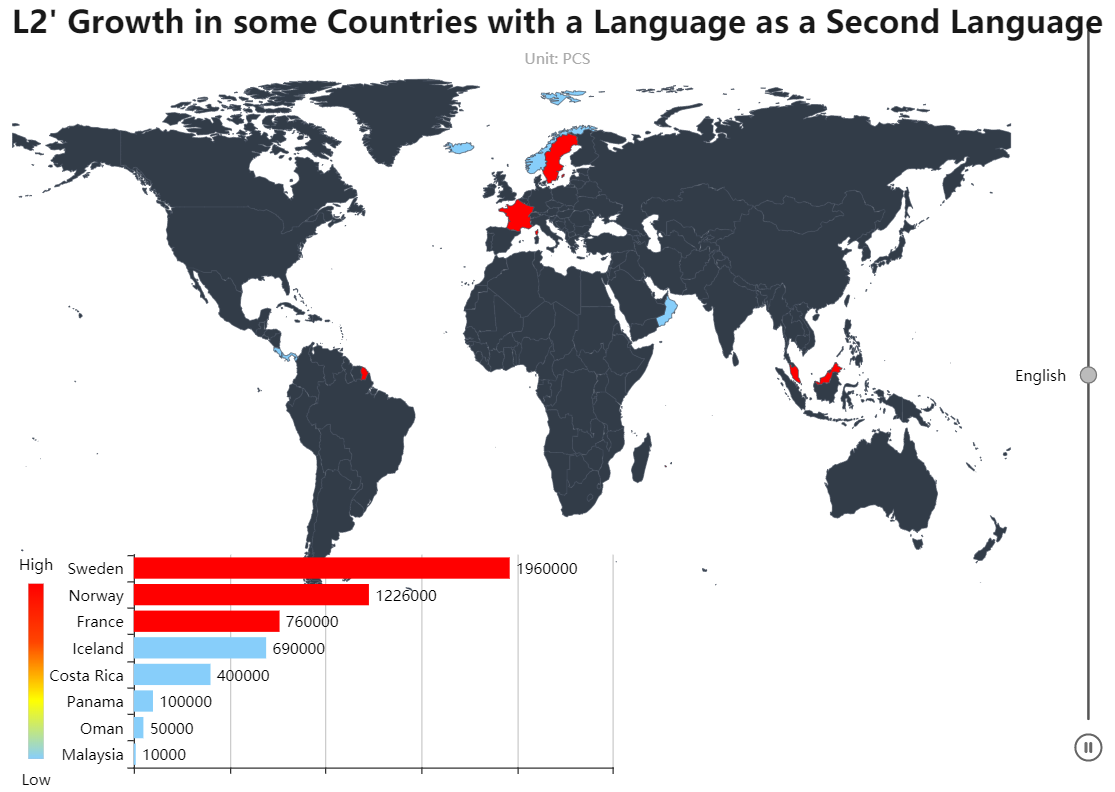
\includegraphics[width=1\linewidth,height=10cm]{figures/english}
	\caption{Geographical distribution of English as a second language in 2067}
	\label{fig:english}
\end{figure}

\noindent Note: The color column changes upward, representing the increase in the number of more.

 From the comparison between the above figure and the known geographical distribution in 2017, we can see that the countries currently speaking English as the second language are mainly located in four regions:Western and Central European countries (Sweden, Norway, France, Iceland, Poland), Malaysia, Central American countries, East African countries (Egypt, Sudan, Cameroon).The number of L2 speakers in English in 2017 was 611 million, rising to 1.147 billion in 2067, an increase of 536 million in the number of speakers of L2 in 50 years.Of these, countries rank the highest to the lowest in the country: 1,976,000(Sweden)> 1,226,600(Norway)> 76,000(France)> 69,000 (Iceland) > 400,000 (Costa Rica) > 100,000.
\par Analysis of the geographical distribution of changes:
\begin{itemize}
	\item The growth of the three North West European countries, Switzerland, Norway and France, showed the most noticeable changes. The growth rates of these three countries were all above 700,000. In addition, some Nordic countries also saw an increase in their numbers;
	\item The number of Central American countries and the Malay archipelago has been significantly reduced;
	\item African countries have a net negative net migration, so few people have used English as their second language. 
\end{itemize} 

\par The figure below is the geographical distribution of Spanish as a second language:

\begin{figure}[H]
	\centering
	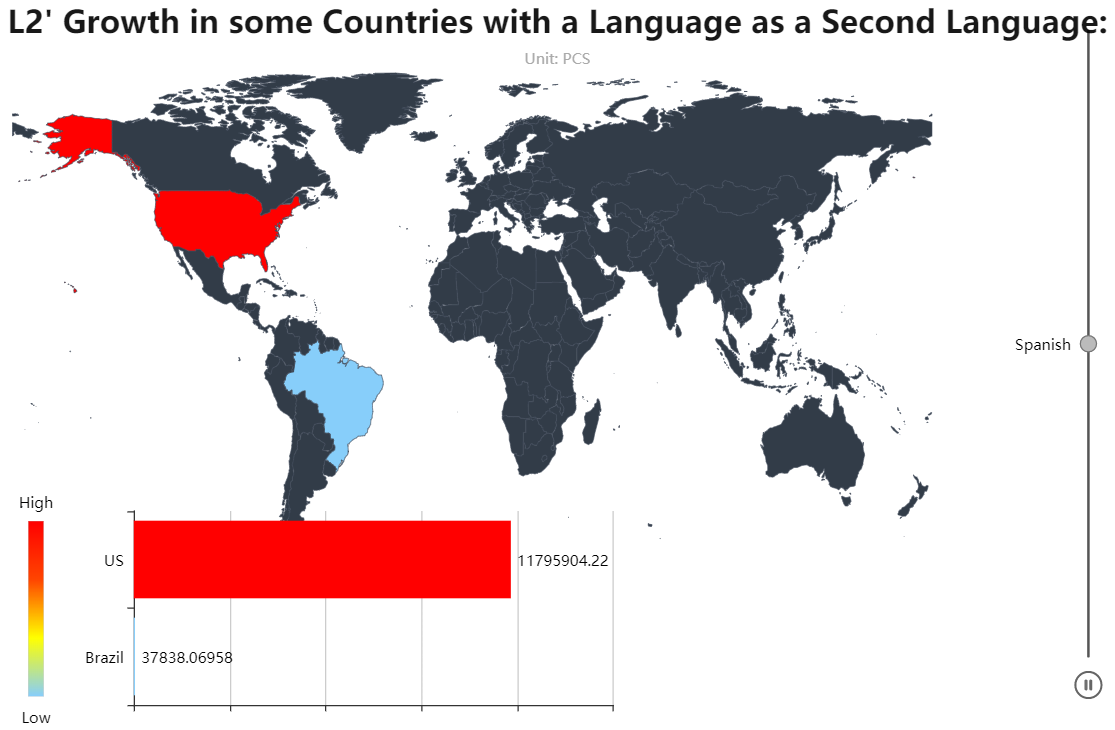
\includegraphics[width=1\linewidth,height=10cm]{figures/Spanish}
	\caption{Geographical distribution of Spanish as a second language in 2067}
	\label{fig:spanish}
\end{figure}

\par From the above figure and the known geographical distribution in 2017, we can see that: Currently, countries with Spanish as their second language are mainly based on estimates in the United States and Brazil. The number of L2 users in Spain by 2067 was 152 million, an increase of 62 million compared with 90 million in 2017. Affected by the number of net immigrants, the migration to the United States is about 11.7 million more than that of Brazil, so the color shown in the United States is red and the color shown in Brazil is light blue. 

\subsection{the location of the new international office}

\noindent Effective language can promote the development of business, so we consider choosing to develop the company's business in a region where language has potential for development. Based on the results of the first part of the question, we build a model of linguistic performance evaluation that evaluates and ranks the performance of languages to determine the preferred locations for the six international offices.

\par First of all, we need to determine the evaluation index to build the evaluation model.The evaluation indicators are selected from the five categories of geography, economy, total number of languages spoken in one language (inc.pl1 \& pl2), information output and quality of languages, and the situation in which the international organizations use the language.We consider that many of the indicators are economic-related and not directly related to language.Therefore, we think that the indicator of the economy is directly related to the dominant language of the economy. What needs to be pointed out is that for a certain language we only count the countries where the native language is in this language and the population exceeds 10million.
\par Then, as explained in the Problem Analysis section, we set up a language performance evaluation (LII) model.Taking into account that the indicators have different dimensions, we quantify each indicator to [0,1], calculate the language influence score and rank them. According to the rankings, the cities were specifically identified based on the state of the economy at the national level in the language and the reasons for the changes in the locations of the six new international offices in the short and long term were analyzed.Finally, consider the changes in the nature of global communications, the widespread use of electronic media, more and more convenient and accurate translation software, making language constraints reduced,multinational corporations may consider opting to set up offices in less than six places, giving the location of the office and describing the corresponding reasons.

\subsubsection{Language Effectiveness Evaluation Model(LII)} 

\noindent In order to evaluate the linguistic influence more reasonably, we have been inspired by reference [7] to propose the language influence Index (LII) model.Language Influence Index (LII) selects 14 indicators to measure the influence of language from 5 aspects. The 14 indicators we choose are as follows:

\begin{enumerate}
	\item[1)] \textbf{Area: Extensive geographical advantage of language diffusion}
	\par \textbf{Number of countries that speak the language :*}This indicator relates to the number of countries or regions that use this language as their mother tongue and some also include this language as a second language.The greater number of countries that use this language as a mother tongue or a second language demonstrates that the distribution of language is more adequate and the greater the international influence of the language.We define the mapping rules for this metric as follows: If a language is "dominant", the metric is valued of 1; conversely, if it is a "minority", its value is 0.5.
	\par \textbf{National Land area:}By looking at the data [7], we know that the size of the land area can be approximated to measure a country's linguistic exclusiveness, which in turn affects the country's "dominant" language's international influence.
	\par \textbf{Inbound tourists:}This indicator mainly reflects the number of overnight visitors to the country. Mainly by the language group's culture to attract, and understand a culture must learn the culture carrier - language.
	
	\item[2)] \textbf{Economy strength: Language plays an important role in economic life}
	\par \textbf{GDP:}The level of economic development of a language group has an obvious and self-evident important influence on the international influence of the language. Therefore, we include it in the indicator range.
	\par \textbf{GDP per capita*:}This indicator reflects the overall level of development of a region and can characterize the attraction of the region to those who have the will to emigrate.
	\par \textbf{Exports: }When exports are larger than imports, trade surpluses often appear and trade surpluses can enhance the international influence of regional languages.
	
	\item[3)] \textbf{Language speakers: Direct Impact factors}
	\par \textbf{Native speakers and Second language (L2) speakers:*} These two indicators are based on the first part of the forecasting model, and have a direct impact on the linguistic impact assessment and analysis.
	
	\item[4)] \textbf{Knowledge and media: An important channel for language communication}
	\par\textbf{Internet use language: } The Internet has an important influence on the spread of language influence. With the globalization of information, the possession of a language in the Internet plays an important role in developing the international influence of the language.
	\par \textbf{Higher education uses language:}The language used in a national education and teaching school, especially the language used in higher education, and outstanding education will attract a large number of overseas students and thus promote the conversion of a foreign language into a second language.
	
	\item[5)] \textbf{International use: Language in the international recognition}
	\par \textbf{International organizations:}We consider that some international organizations in the world play an important role in promoting the spread of linguistic influence. Therefore, we think the index as a measure. Here we consider the IMF, UN, WB and other 10 international organizations (index of 10 organizations).For example, if a language is the official language of the International Monetary Fund, the indicator picks up the value of 1, otherwise 0. From Wikipedia, you can find the official language used by each international organization.
	
\end{enumerate}

\par To show the structure of our model more clearly, here's a diagram of the Language Influence Index (LII):

\begin{figure}[H]
	\centering
	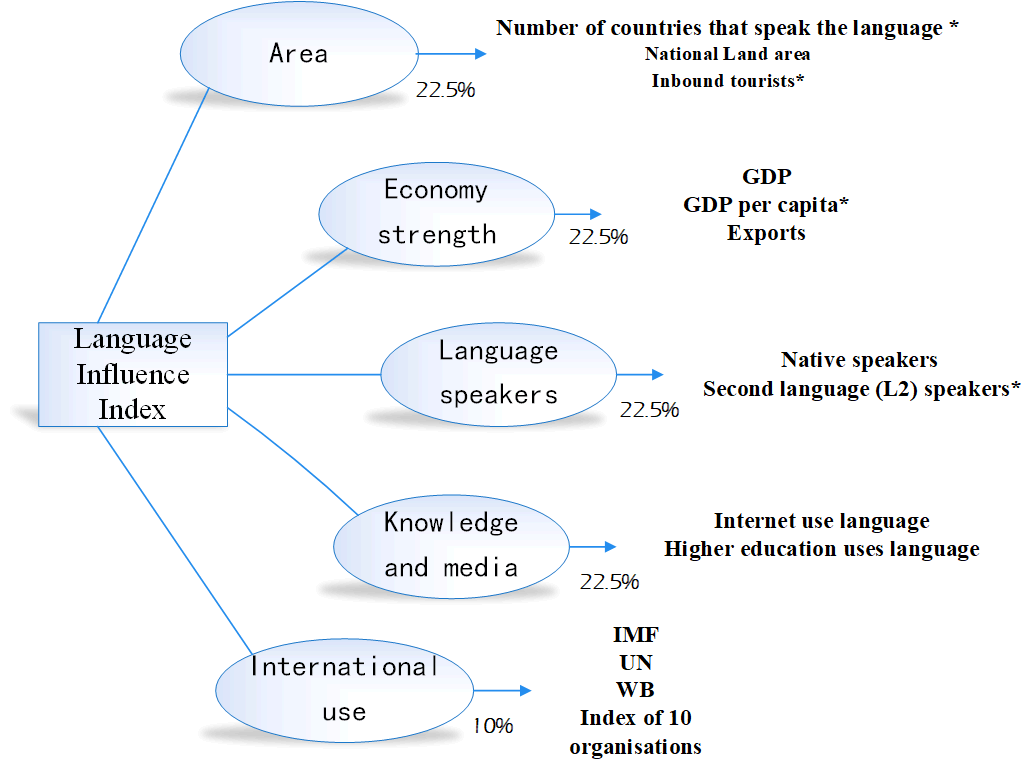
\includegraphics[width=0.7\linewidth]{figures/chart}
	\caption{Language Influence Index Structure chart}
	\label{fig:chart}
\end{figure}

\par \textbf{LII model construction process is as follows:}

\begin{enumerate}
	\item[1)] \textbf{Determination of the weight of influence index}
	\par Assuming that the overall weight of the indicator is 1, when considering the five aspects of the promotion of the international influence of the language, the indicators in the first four categories together account for 0.9, and the weight in the final category accounts for 0.1. At the same time, the weight of indicators in each aspect is inversely proportional to the number of indicators.The definition uses ${\omega _m}$ for the weight of each indicator and $m$ for the mth indicator:
	\begin{equation}
	{\omega _m} = \left\{ \begin{array}{l}
	\frac{{0.9}}{4} \times \frac{1}{3} = 0.075{\rm{          }} \quad m \in Area,Economy\;{\rm{ }}strength;m = 1,2,3,4,5,6{\rm{   }}\\
	\\
	\frac{{0.9}}{4} \times \frac{1}{2} = 0.1125{\rm{        }}\quad m \in Language\;{\rm{ }}speakers,Knowledge\;{\rm{ }}and\;{\rm{ }}media\\
	\\
	{\rm{                                  }} \quad \quad \quad \quad \quad \quad \quad \quad  m{\rm{ = }}7,8,910\\
	\\
	0.1 \times \frac{1}{4} = 0.025{\rm{           }}\quad \in International\;{\rm{ }}use;m = 11,12,13,14
	\end{array} \right. \label{aa1}
	\end{equation}
	
	\item[2)] \textbf{the normalization of language indicators}
	\par Since the dimensions of each indicator are not consistent, in order to unify the calculation, we normalize the indicators and map their values to [0,1].The process is as follows: Define the value of the $m$ indicator corresponding to the $j$th language to be $V_m^j$, then normalize by the following formula:
	
	\begin{equation}
	S_m^j = \frac{{V_m^j}}{{\max \left\{ {V_m^1,V_m^2,...,V_m^j} \right\}}}{\rm{        }}\quad j \in [1,20],j\;{\rm{ is\; an\; integer}}\label{aa1}
	\end{equation}
	
	\par Among them, ${s_m}^j$ is the m-th index normalized result, ${s_m}^j \in [0,1]$.
	
	\item[3)] \textbf{the international influence of language}
	\par The $j$th language was quantified as the score of [0,1] score interval and the score  of the international influence weighted by the weight of the $j$th language, ie, the score of language influence. The formula for calculating the total language score is:
	 
	 \begin{equation}
	 {S^j} = \sum\limits_{m = 1}^{15} {({P_m} \times S_m^j)} {\rm{       }}\quad m\;{\rm{ is\; an\; integer}} \label{aa1}
	 \end{equation}
	 \par Of which: ${s^j}$ indicates the total international influence in the $j$th language.
	
\end{enumerate}

\par According to the above formula and historical data, we can draw the scores and rankings of mainstream languages in the world from 2012 to 2014:


% Table generated by Excel2LaTeX from sheet 'Sheet2'
\begin{table}[H]
	\centering
	\caption{2012-2013 scores of some languages and rankings}
	 \scalebox{0.87}[0.87]{%
	\begin{tabular}{p{4.11em}rrrrrr}
		\toprule
		\multicolumn{1}{c}{\multirow{2}[4]{*}{\backslashbox[0pt][l]{Language}{Time}}} & \multicolumn{2}{c}{2012} & \multicolumn{2}{c}{2013} & \multicolumn{2}{c}{2014} \\
		\cmidrule{2-7}    \multicolumn{1}{c}{} & \multicolumn{1}{p{4.11em}}{Score} & \multicolumn{1}{p{4.11em}}{Rank} & \multicolumn{1}{p{4.055em}}{Score} & \multicolumn{1}{p{4.055em}}{Rank} & \multicolumn{1}{p{4.055em}}{Score} & \multicolumn{1}{p{4.055em}}{Rank} \\
    \midrule
	English & 0.853  & 1     & 0.853  & 1     & 0.752  & 1 \\
	\midrule
	Chinese & 0.416  & 2     & 0.401  & 2     & 0.318  & 2 \\
	\midrule
	French & 0.301  & 5     & 0.302  & 4     & 0.200  & 7 \\
	\midrule
	Spanish & 0.398  & 3     & 0.401  & 3     & 0.307  & 3 \\
	\midrule
	Arabic & 0.278  & 7     & 0.275  & 7     & 0.202  & 6 \\
	\midrule
	Russian & 0.226  & 8     & 0.224  & 8     & 0.140  & 9 \\
	\midrule
	German & 0.280  & 6     & 0.276  & 6     & 0.268  & 5 \\
	\midrule
	Japanese & 0.179  & 9     & 0.180  & 9     & 0.153  & 8 \\
	\midrule
	Portuguese & 0.145  & 10    & 0.142  & 10    & 0.137  & 10 \\
	\midrule
	Hindi & 0.305  & 4     & 0.301  & 5     & 0.301  & 4 \\
	\bottomrule
	\end{tabular}%
}
	\label{tab:012}%
\end{table}%

 As can be observed in the above table, the more rankings indicate the higher the influence of the language. LII model calculates the language impact score each year the language score will be some basic changes. For example, French ranked fifth from 2012, ranking up one place in 2013 and down three places in 2014; English has been the number one language influence in these three years, with the weakest influence in Portugal.

\subsubsection{Establishment of six new international offices} 
\noindent The key factors to consider when adding a new office are: Regional Language effectiveness. In fact, the newly added international offices are generally located in economically developed and easily accessible cities, so we have only given the preferred language zone for the office, which can be decided by the multinational company for the specific location of the new office. At the same time, pay attention to the fact that the two countries in the United States and China have set up their own offices, so no additional office will be set up.
\par In this paper, we simplify: Assuming that the country with the largest number of native speakers of a language is the country where the new international office is located. The capital is chosen as the preferred address from that country.
\par The table below shows the rankings of the world's major languages in terms of their language performance over a 50-year period, sorting out the ranking data for each decade:

% Table generated by Excel2LaTeX from sheet 'Sheet2'
\begin{table}[H]
	\centering
	\caption{Change of language performance rankings every decade}
		 \scalebox{0.87}[0.87]{%
	\begin{tabular*}{40em}{@{\extracolsep{\fill}}ccccccc}
		\toprule
		\multicolumn{1}{r}{\backslashbox[0pt][l]{Language}{Year}} & 2017  & 2027  & 2037  & 2047  & 2057  & 2067 \\
		\midrule
		English & 1     & 1     & 1     & 1     & 1     & 1 \\
		\midrule
		Chinese & 2     & 2     & 2     & 2     & 2     & 2 \\
		\midrule
		French & 3     & 3     & 4     & 4     & 4     & 4 \\
		\midrule
		Spanish & 4     & 4     & 3     & 3     & 3     & 3 \\
		\midrule
		Arabic & 5     & 5     & 5     & 5     & 6     & 6 \\
		\midrule
		Russian & 6     & 6     & 6     & 6     & 5     & 5 \\
		\midrule
		German & 7     & 7     & 7     & 7     & 7     & 8 \\
		\midrule
		Japanese & 8     & 9     & 9     & 10    & 10    & 10 \\
		\midrule
		Portuguese & 9     & 8     & 8     & 8     & 9     & 9 \\
		\midrule
		Hindi & 10    & 10    & 10    & 9     & 8     & 7 \\
		\bottomrule
	\end{tabular*}%
}
	\label{tab:Change}%
\end{table}%

\par In the short term (10 years): Top 6 languages and 2017 rankings have not changed.The six cities identified by rankings are: \textbf{London, England / Paris, France / Madrid, Spain/Dammam, Saudi Arabia / Moscow, Russia and Berlin, Germany.}
\par From the long-term (50 years) point of view: English, Chinese rankings have not changed; Spanish, Russian ranking rose one; Arabic, French, German down one place; Hindi influence is on the rise 2 to 3 ranks higher; Japanese and Portuguese have been the last to influence. If we are to set up a new international office by 2067, the top six countries will remain unchanged. However, we can see the trend of development. The impact of Hindi is gradually increasing, and the market has great potential for development. So six additional international offices are located in:\textbf{ London, England / Madrid, Spain / Paris, France / Moscow, Russia / Dammam, Saudi Arabia and New Delhi, India.}

\subsubsection{Changes in the nature of the global communications site impact}
\noindent With the popularization of the Internet and the development of new media, the two places geographically far away can still communicate with each other. Even if the language barrier is not available, they can travel around the world with translation software and learn the culture. So consider setting up fewer than six new international offices.
\par The whole earth can be subdivided into six plates. If multinational companies can set up international offices on every continent, each continent has its unique resources. According to the UN future world population forecast trend report and the model established in this paper and the results obtained: India will surpass China as the world's largest population in 2022 and Africa and Asia will become densely populated in the future. Europe, North America, Oceania is owned by the densely populated areas of developed countries. South America, Brazil, Chile, the second language prominent.
\par Therefore, in addition to North America, New York, USA and Shanghai, Asia, China, four more new international offices can be established: \textbf{Oceania Australia Sydney / Africa Nigeria Nigeria Abuja / South America Brazil Brasilia / Europe UK London.}

 
 % 模型
%\section{Conclusions}
According to our model, the trend of language development can be reflected in two aspects: the number of language speakers and the regional differences in languages.The location of the new international office is based on the key factors: the effectiveness of the language.
\par In the part of prediction of the trend of languages,we can obtain the change of the total number of speakers of the mainstream languages in the world(Shown in Fig.1), the variations of the number of native speakers in the mainstream languages(Shown in Fig.2),languages of top ten(both native speakers and total speakers) and their ranks in fifty years(see table3).What's more, We find that ranked currently in the top ten languages in the future rankings remain in the top ten, but the specific rankings changethe total number of speakers of English exceeds the number of speakers of Chinese in 2045, when the total population of the former reach 1,432.163 million.As for the part of geographical distribution of language speakers, we obtain that the Arabic speakers account for 50.13\% of the total Arabic speaker in 2048.Additionally, the most powerful growth is in Spanish.
\par In the part of siting in international offices,we build an evaluation model of language effectiveness. Based on this model, we examine the effectivenesse of the mainstream language over time. Further, we determine the language zones to be selected for the new international office based on the performance ranking of the language.Based on the results of our modeling, we find no significant differences in the rankings of language performance in the short term and long term,so there is no change in the construction plan for the new office.When we assume that we can capture the penetration of regional Internet and that the multinational companies have web services.We obtain the higher the Internet penetration rate in a given area, the lower the need to have an office there.Therefore, we propose to reduce the number of offices in developed regions and consider setting up offices in areas with great potential such a some areas of Africa % 结论
\section{Sensitivity analysis of the model}
\noindent
In the language performance evaluation model, the weight of each indicator is defined with reference to relevant information. For this we can compare the last language rankings with big changes by changing the index weights. Discuss two new ways to specify weights:

\begin{itemize}
	\item 5 indicators equally, each 0.2.
	\item Considering the actual situation, the influence of the area and the international use on the language is weak, taking 0.1.The remaining three factors bisect 0.8.
\end{itemize}


% Table generated by Excel2LaTeX from sheet 'Sheet1'
\begin{table}[H]
	\centering
	\caption{Indicator weighting table for three different scenarios}
	\scalebox{0.87}[0.87]{%
	\begin{tabular}{cp{5em}p{5em}p{5em}p{5em}p{6em}}
		\toprule
		 & Area & Economy strength & Language speakers & Knowledge and media &International use\\
		\midrule
		original plan & 0.225 & 0.225 & 0.225 & 0.225 & 0.1 \\
		\midrule
		Plan 1 & 0.25  & 0.25  & 0.25  & 0.25  & 0.25 \\
		\midrule
		Plan 2 & 0.1   & 0.27  & 0.27  & 0.27  & 0.1 \\
		\bottomrule
	\end{tabular}%
}
	\label{tab:addlabel}%
\end{table}%


Use the score calculation method in 5.2.1 to calculate the rankings of the language performance scores of three different weights. The ranking table is given in the appendix.It can be seen that the rankings of the first seven languages do not change, and the rankings of the latter four languages are slightly changed. Therefore, we can draw a conclusion that the language performance evaluation model we established has good stability. % 灵敏度分析
\section{Conclusions}
According to our model, the trend of language development can be reflected in two aspects: the number of language speakers and the regional differences in languages.The location of the new international office is based on the key factors: the effectiveness of the language.
\par In the part of prediction of the trend of languages,we can obtain the change of the total number of speakers of the mainstream languages in the world(Shown in Fig.1), the variations of the number of native speakers in the mainstream languages(Shown in Fig.2),languages of top ten(both native speakers and total speakers) and their ranks in fifty years(see table3).What's more, We find that ranked currently in the top ten languages in the future rankings remain in the top ten, but the specific rankings changethe total number of speakers of English exceeds the number of speakers of Chinese in 2045, when the total population of the former reach 1,432.163 million.As for the part of geographical distribution of language speakers, we obtain that the Arabic speakers account for 50.13\% of the total Arabic speaker in 2048.Additionally, the most powerful growth is in Spanish.
\par In the part of siting in international offices,we build an evaluation model of language effectiveness. Based on this model, we examine the effectivenesse of the mainstream language over time. Further, we determine the language zones to be selected for the new international office based on the performance ranking of the language.Based on the results of our modeling, we find no significant differences in the rankings of language performance in the short term and long term,so there is no change in the construction plan for the new office.When we assume that we can capture the penetration of regional Internet and that the multinational companies have web services.We obtain the higher the Internet penetration rate in a given area, the lower the need to have an office there.Therefore, we propose to reduce the number of offices in developed regions and consider setting up offices in areas with great potential such a some areas of Africa % 结论
\section{Strengths and weaknesses}
\subsection{Strengths}
\begin{itemize}
	\item \textbf{Improve the existing model}
\newline Existing indicators of linguistic influence assessment model change and the evaluation of linguistic effectiveness that is more suitable for solving this problem are improved. To quantify the linguistic influence of the abstract description to a fraction of [0,1] and calculate the language score to provide a reasonable basis for the new international office location
	\item \textbf{Good flexibility}
\newline To study this problem, two main models are established: the non-equidistant GM (1,1) prediction model and the language performance evaluation model (LII). The former model can be used for other forecasting problems. The latter model can be extended to the evaluation problem. The model is more flexible and can be transformed into a solution to other practical problems
	\item \textbf{youdian}
	
	\item \textbf{youdian}
	
\end{itemize}

\subsection{weaknesses}

\begin{itemize}
	\item \textbf{Inaccuracy} \newline
	In the first part of the forecast of the development trend of the global language, due to the time factor analysis did not use multivariate analysis, nor did it fully consider the background of the factors. Based on the actual data we found, we used the predictive model to predict the data, which is a little bit different from the actual situation
	\item \textbf{Simplifying assumptions}
	\newline In the establishment of a population migration model, the simplification assumption assumes that only the net migration population is considered, the gravitation analysis for the population movements is not enough, and the geographical distribution and proliferation of the second language caused by the actual population flows in terms of the number of refugees, economic factors and policy factors are not tapped.
	\item \textbf{Lack of data}
	\newline 
	The census and statistics of the global language population are extremely difficult and complex tasks. This question is required to collect a lot of data, the subject only gives a year of data, you must have nearly 10 years of data to make long-term forecasts. We collect less valid data, which leads to inaccurate results of the forecasting model.
\end{itemize}
\section{Future Improvements}

\begin{itemize}
\item Since we did not fully consider the background factors given in the subject when we set up the forecasting model, we only make a prediction based on the data of the linguistic population itself, and the error between this forecast and the actual situation is relatively large. The main reason is that less than the relevant data cannot be collected. If we can get the historical data of 5-10 years from the relevant factors and we can correct the predicted values through the relevant factor analysis, then the result of our model will be more accurate.\\
\item For the change of linguistic population on geographical distribution, we may have some limitations to simplify the analysis and to study only the changes of the net migration population under the research of the state. We believe that we can also analyze the language flow direction from the discrepancy or gravity of any two languages to establish the "language distance" model or the gravity model. Thus, we can draw a directed graph of geographical distribution of the number of second-language mainstream in the world and more vividly analyze the impact of the mode of population migration on geographical distribution of languages.
\end{itemize} %进一步提高
\input{paper/Memorandum} % 说明书
% =================================================================
%引用别人的成果或其他公开的资料(包括网上资料)必须按下列方式在正文引用处和参考文献中明确列出。正文引用处用方括号标示参考文献的编号,如[1]、[3]等;引用书籍必须指出页码。参考文献按正文中的引用次序列出,其中书籍的表述方式为:
%[编号] 作者,书名,出版地:出版社,出版年。
%参考文献中期刊杂志论文的表述方式为:
%[编号] 作者,论文名,杂志名,卷期号:起止页码,出版年。
%参考文献中网上资源的表述方式为:
%[编号] 作者,资源标题,网址,访问时间(年月日)。

\begin{thebibliography}{99}
	\addcontentsline{toc}{section}{References} % 在目录中添加参考文献
		
%	\bibitem{1}United Nations,Feature Films and Cinema Data, \url{http://uis.unesco.org/en/topic/feature-films-and-cinema-dat},2/12/2018.

	
	\bibitem{cinemaData}The list of languages by population,https://en.wikipedia.org/wiki/The\_list
	\_of\_languages\_by\_population,February 13, 2018
	\bibitem{gm11}	Dai Wenzhan, Li Junfeng.Study on modeling of non-equidistant GM (1, 1) model [J] .Systems Engineering -Theory \& Practice, 2005, 25 (9): 89-93.
	\bibitem{gray}Chen Youliang.Non-equidistant gray forecasting method and its application in rock mechanics and engineering [J] .Systems Engineering -Theory \& Practice, 2003, 23 (11): 130-134.
	\bibitem{travel}The second language other than the mother tongue of the countries in the world is counted,	http://www.mafengwo.cn/travel-news/220416.html,February 13, 2018
	\bibitem{undata}UN immigration data,	https://esa.un.org/.../WPP2017\_MIGR\_F02\_NET
	\_NUMBER\_OF\_MIGRAN,February 13, 2018
	\bibitem{mapdata}	http://gallery.echartsjs.com/editor.html?c=xSyKKAw97l
	\bibitem{influential}	LANGUAGE INFLUENCE INDEX,Which are the world’s most influential languages? Kai L. Chan, PhD, 2018.02.11

\end{thebibliography}
%\upcite{cinemaData} % 电影数据
%\upcite{gm11} % %陈勇2005非等间距序列的灰色模型的程序实现
%\upcite{mapdata} % 画图引用
%\upcite{archive} % 民族志
%\upcite{Dataset}% 民族志购买的数据
%\upcite{undata} %联合国数据
%\upcite{influential}%最有影响力的语言
%\upcite{wiki} %维基百科

%\newpage
%\bibliography{books}
%
\begin{appendices}
	
	\section*{Code appendix} % \section*{title} 不加入目录
	
	Here are simulation programmes we used in our model as follow.\\
	
	
	
	\textbf{\textcolor[rgb]{0.98,0.00,0.00}{MATLAB code of non-equal spacing of GM (1,1) :}}
	\lstinputlisting[language=matlab]{./code/L2.m}

	\section*{Charts and Figures}
	% Table generated by Excel2LaTeX from sheet 'Sheet2'
	\begin{table}[H]
		\centering
		\caption{ The second language is mainly used in countries / regions}
		\begin{tabular}{llp{4cm}p{4cm}}
			\toprule
			language & Asian & Europe & Oceania \\
			\midrule
			Chinese &       &       & Australian \\
			\midrule
			English &       & Sweden, France, Iceland, Poland &  \\	\midrule
			spanish &       &       &  \\	\midrule
			Arabic &       &       &  \\	\midrule
			Russian &       &Ukraine, Kazakhstan, Uzbekistan,Turkmen&  \\	\midrule
			Bengalese & India&       &  \\	\midrule
			Portuguese &       &       &  \\	\midrule
			French &       &       &  \\	\midrule
			Hausa &       &       &  \\	\midrule
			Turkish &       & Austria,Germany, Bulgaria &  \\	\midrule
			Italian &       &       &  \\
			\bottomrule
			\toprule
			language & North America& South America &  Africa \\
			\midrule
			Chinese &       &       &  \\	\midrule
			English & Central America & & Egypt,Sudan ,Cameroon ,Cameroon \\	\midrule
			spanish & \multicolumn{1}{l}{America} & Brazil &  \\	\midrule
			Arabic &       &       & Ethiopia ,Chad ,Somalia, South Sudan \\	\midrule
			Russian &       &       &  \\	\midrule
			Bengalese &       &       &  \\	\midrule
			Portuguese &       &       &  \\	\midrule
			French & America&       & Mozambique \\	\midrule
			Hausa &       &       & the Nile ,Nigeria \\	\midrule
			Turkish &       &       &  \\	\midrule
			Italian &       & Argentina & Algeria \\	\midrule
			\bottomrule
		\end{tabular}%
		\label{tab:SixContinents}%
	\end{table}%

% Table generated by Excel2LaTeX from sheet 'L1 (Native) Speakers'
\begin{table}[H]
	\centering
	\caption{L1 (Native) Speakers}
	\begin{tabular}{rp{5cm}rrrrrr}
		\toprule
		\multicolumn{1}{l}{Rank} & Language & 2015  & 2009  & 2005  & 2000  & 1996  & 1961 \\
		\midrule
		1     & Chinese, Mandarin  & 848   & 845   & 873   & 874   & 885   & 460 \\
		2     & Spanish  & 399   & 329   & 322.3 & 322.2 & 226   & 140 \\
		3     & English  & 335   & 328   & 312.5 & 308.2 & 305.6 & 250 \\
		4     & Hindi  & 260   & 259.6 & 259.5 & 259.5 & 182   & 65 \\
		5     & Portuguese  & 203   & 178   & 177.5 & 176   & 170   & 75 \\
		6     & Bengali  & 189   & 193.1 & 193.5 & 182.7 & 168.1 & 75 \\
		7     & Russian  & 166   & 144   & 143.2 & 155.3 & 155   & 130 \\
		8     & Japanese  & 128   & 122   & 122.4 & 122.6 & 122.2 & 95 \\
		9     & Javanese  & 84.3  & 84.6  & 75.5  & 75.5  & 75.5  & 45 \\
		10    & German, Standard  & 85.6  & 90.1  & 95.2  & 95.1  & 98    & 100 \\
		11    & Chinese, Wu  & 80.1  & 78.5  & 77.1  & 74.4  & 70.8  & 50 \\
		12    & Korean  & 77.2  & 69.5  & 67.1  & 67    & 65.5  & 46 \\
		13    & French  & 75.9  & 67.8  & 64.8  & 64.7  & 64    & 65 \\
		14    & Telugu  & 74    & 69.8  & 69.7  & 69.7  & 66.5  & 37 \\
		15    & Marathi  & 71.8  & 68.1  & 68    & 68    & 64.8  & 31 \\
		16    & Turkish  & 70.9  & 71.1  & 50.5  & 50.7  & 50.2  & 25 \\
		17    & Tamil  & 68.8  & 65.7  & 66    & 66    & 62    & 32 \\
		18    & Vietnamese  & 67.8  & 68.6  & 67.4  & 67.7  & 66.9  & 24 \\
		19    & Urdu  & 64    & 60.6  & 60.5  & 60.3  & 56.6  & 75 \\
		20    & Italian  & 63.8  & 61.7  & 61.5  & 61.4  & 61.4  & 55 \\
				\bottomrule
	\end{tabular}%
	\label{tab:L1}%
\end{table}%

% Table generated by Excel2LaTeX from sheet 'Sheet1'
\begin{table}[htbp]
	\centering
	\caption{Three different programs of language score ranking}
	\begin{tabular}{cp{3.6cm}p{3.6cm}p{3.6cm}}
		\toprule
		& original plan & Plan 1 & Plan 2 \\
		\midrule
		English & 1     & 1     & 1 \\
		\midrule
		Chinese & 2     & 2     & 2 \\
		\midrule
		French & 3     & 3     & 3 \\
		\midrule
		Spanish & 4     & 4     & 4 \\
		\midrule
		Arabic & 5     & 5     & 6 \\
		\midrule
		Russian & 6     & 6     & 7 \\
		\midrule
		German & 7     & 7     & 5 \\
		\midrule
		Japanese & 8     & 8     & 8 \\
		\midrule
		Portuguese & 9     & 10    & 9 \\
		\midrule
		Hindi & 10    & 9     & 10 \\
		\midrule
		KAZAKH & 11    & 11    & 11 \\
		\bottomrule
	\end{tabular}%
	\label{tab:addlabel}%
\end{table}%


	
\end{appendices} 
% =================================子文件夹设置====================================
\end{document}
